\section{Differential expression analysis}
\label{sec:dea}

Differential expression analysis was performed using the methods described in
\cref{sec:material_dea}: DESeq2 and \gls{ciriquant}.
In the following sections of this chapter, the results of the differential
expression analysis are presented.

\subsection{\Glspl{crna} associated with estrogen receptor expression}

In order to identify potential markers of estrogen levels, the expression of
the \gls{esr1} gene (described in \cref{sec:esr1}) was used as a proxy.
As \gls{ciriquant} does not support the differential expression along a
continuous variable, only the results obtained using DESeq2 are presented here.
As shown in \cref{fig:esr1_volcano}, the differential expression analysis
revealed a large number of \glspl{crna} significantly associated with the
expression of \gls{esr1}.
The functional enrichment analysis of the host genes of these \glspl{crna} is
shown in \cref{fig:esr1_go_terms}.

\begin{figure}[H] \begin{tabular}{cc} \begin{subfigure}{0.5\textwidth}
                 \centering

                 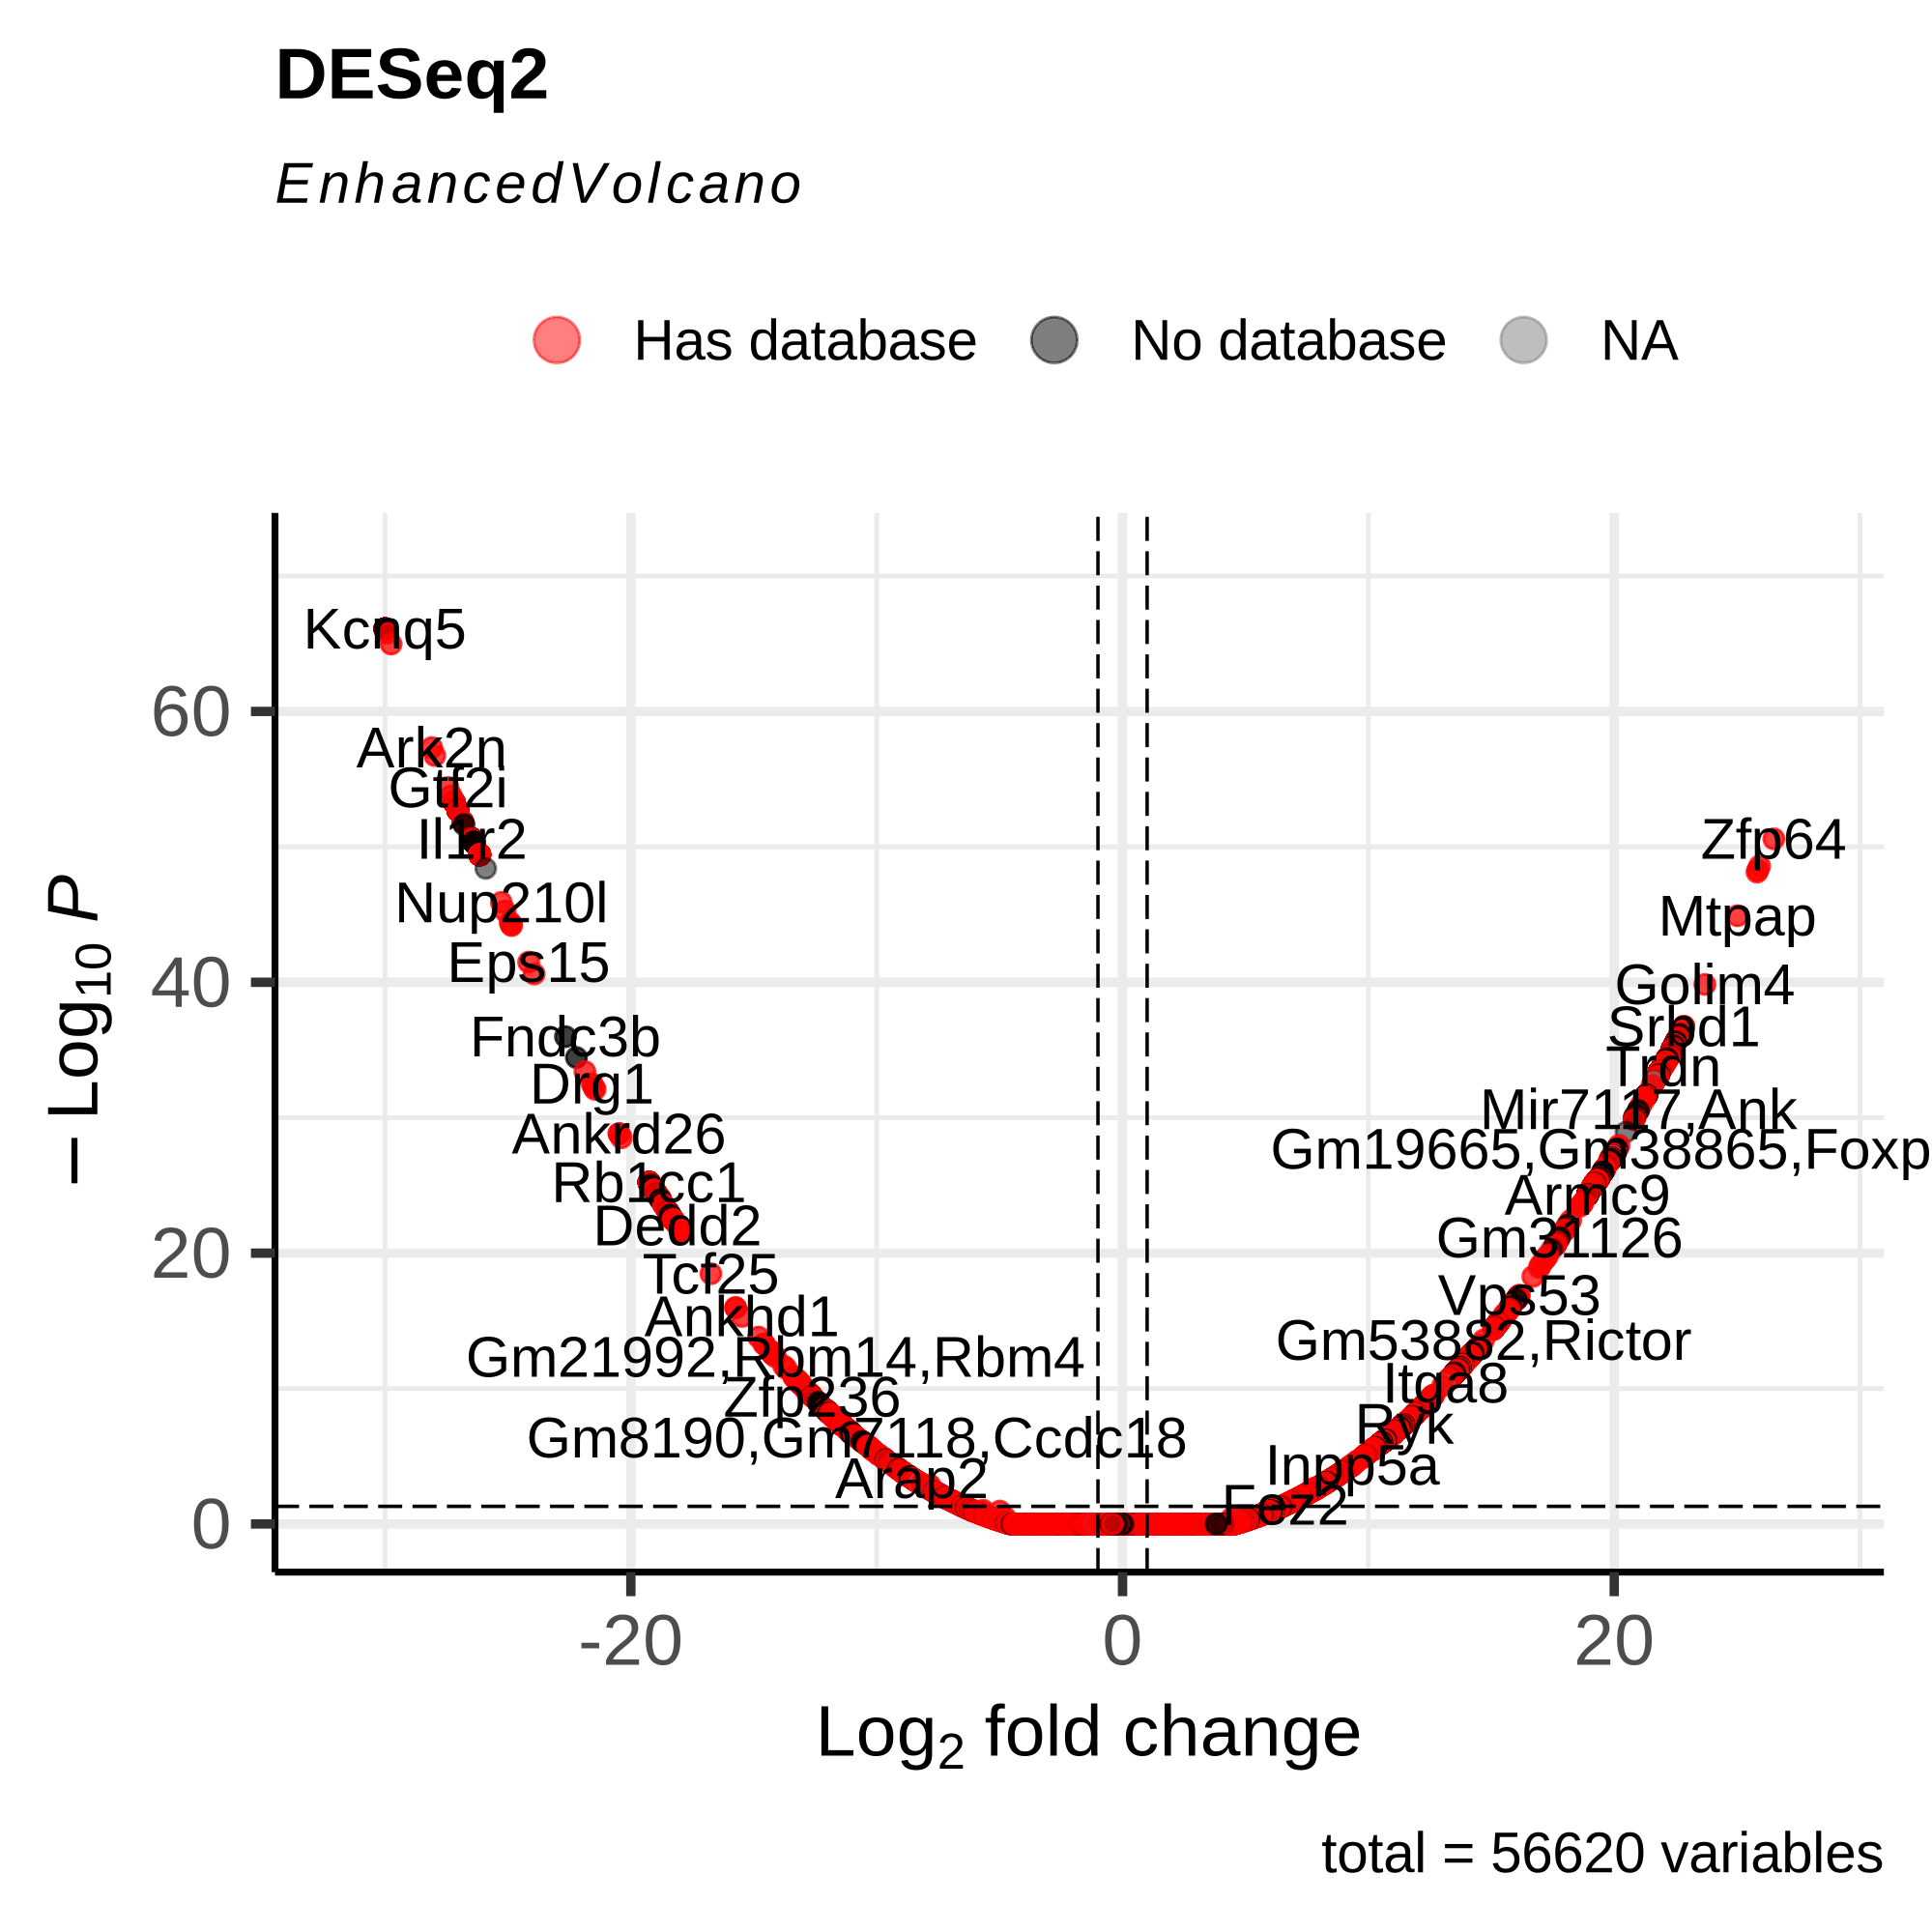
\includegraphics[width=\linewidth]{chapters/4_results_and_discussion/figures/dea/deseq2/esr1/volcano.png}
                 \caption{Volcano plot based on differential expression
                     analysis using DESeq2.
                     Coloring is based on the presence of a supporting database entry in any of the
                     used databases.
                     The labels represent the host genes of the respective \glspl{crna}.
                     Not all labels are shown for better readability.
                 } \label{fig:esr1_volcano} \end{subfigure}
        \begin{subfigure}{0.5\textwidth} \centering

            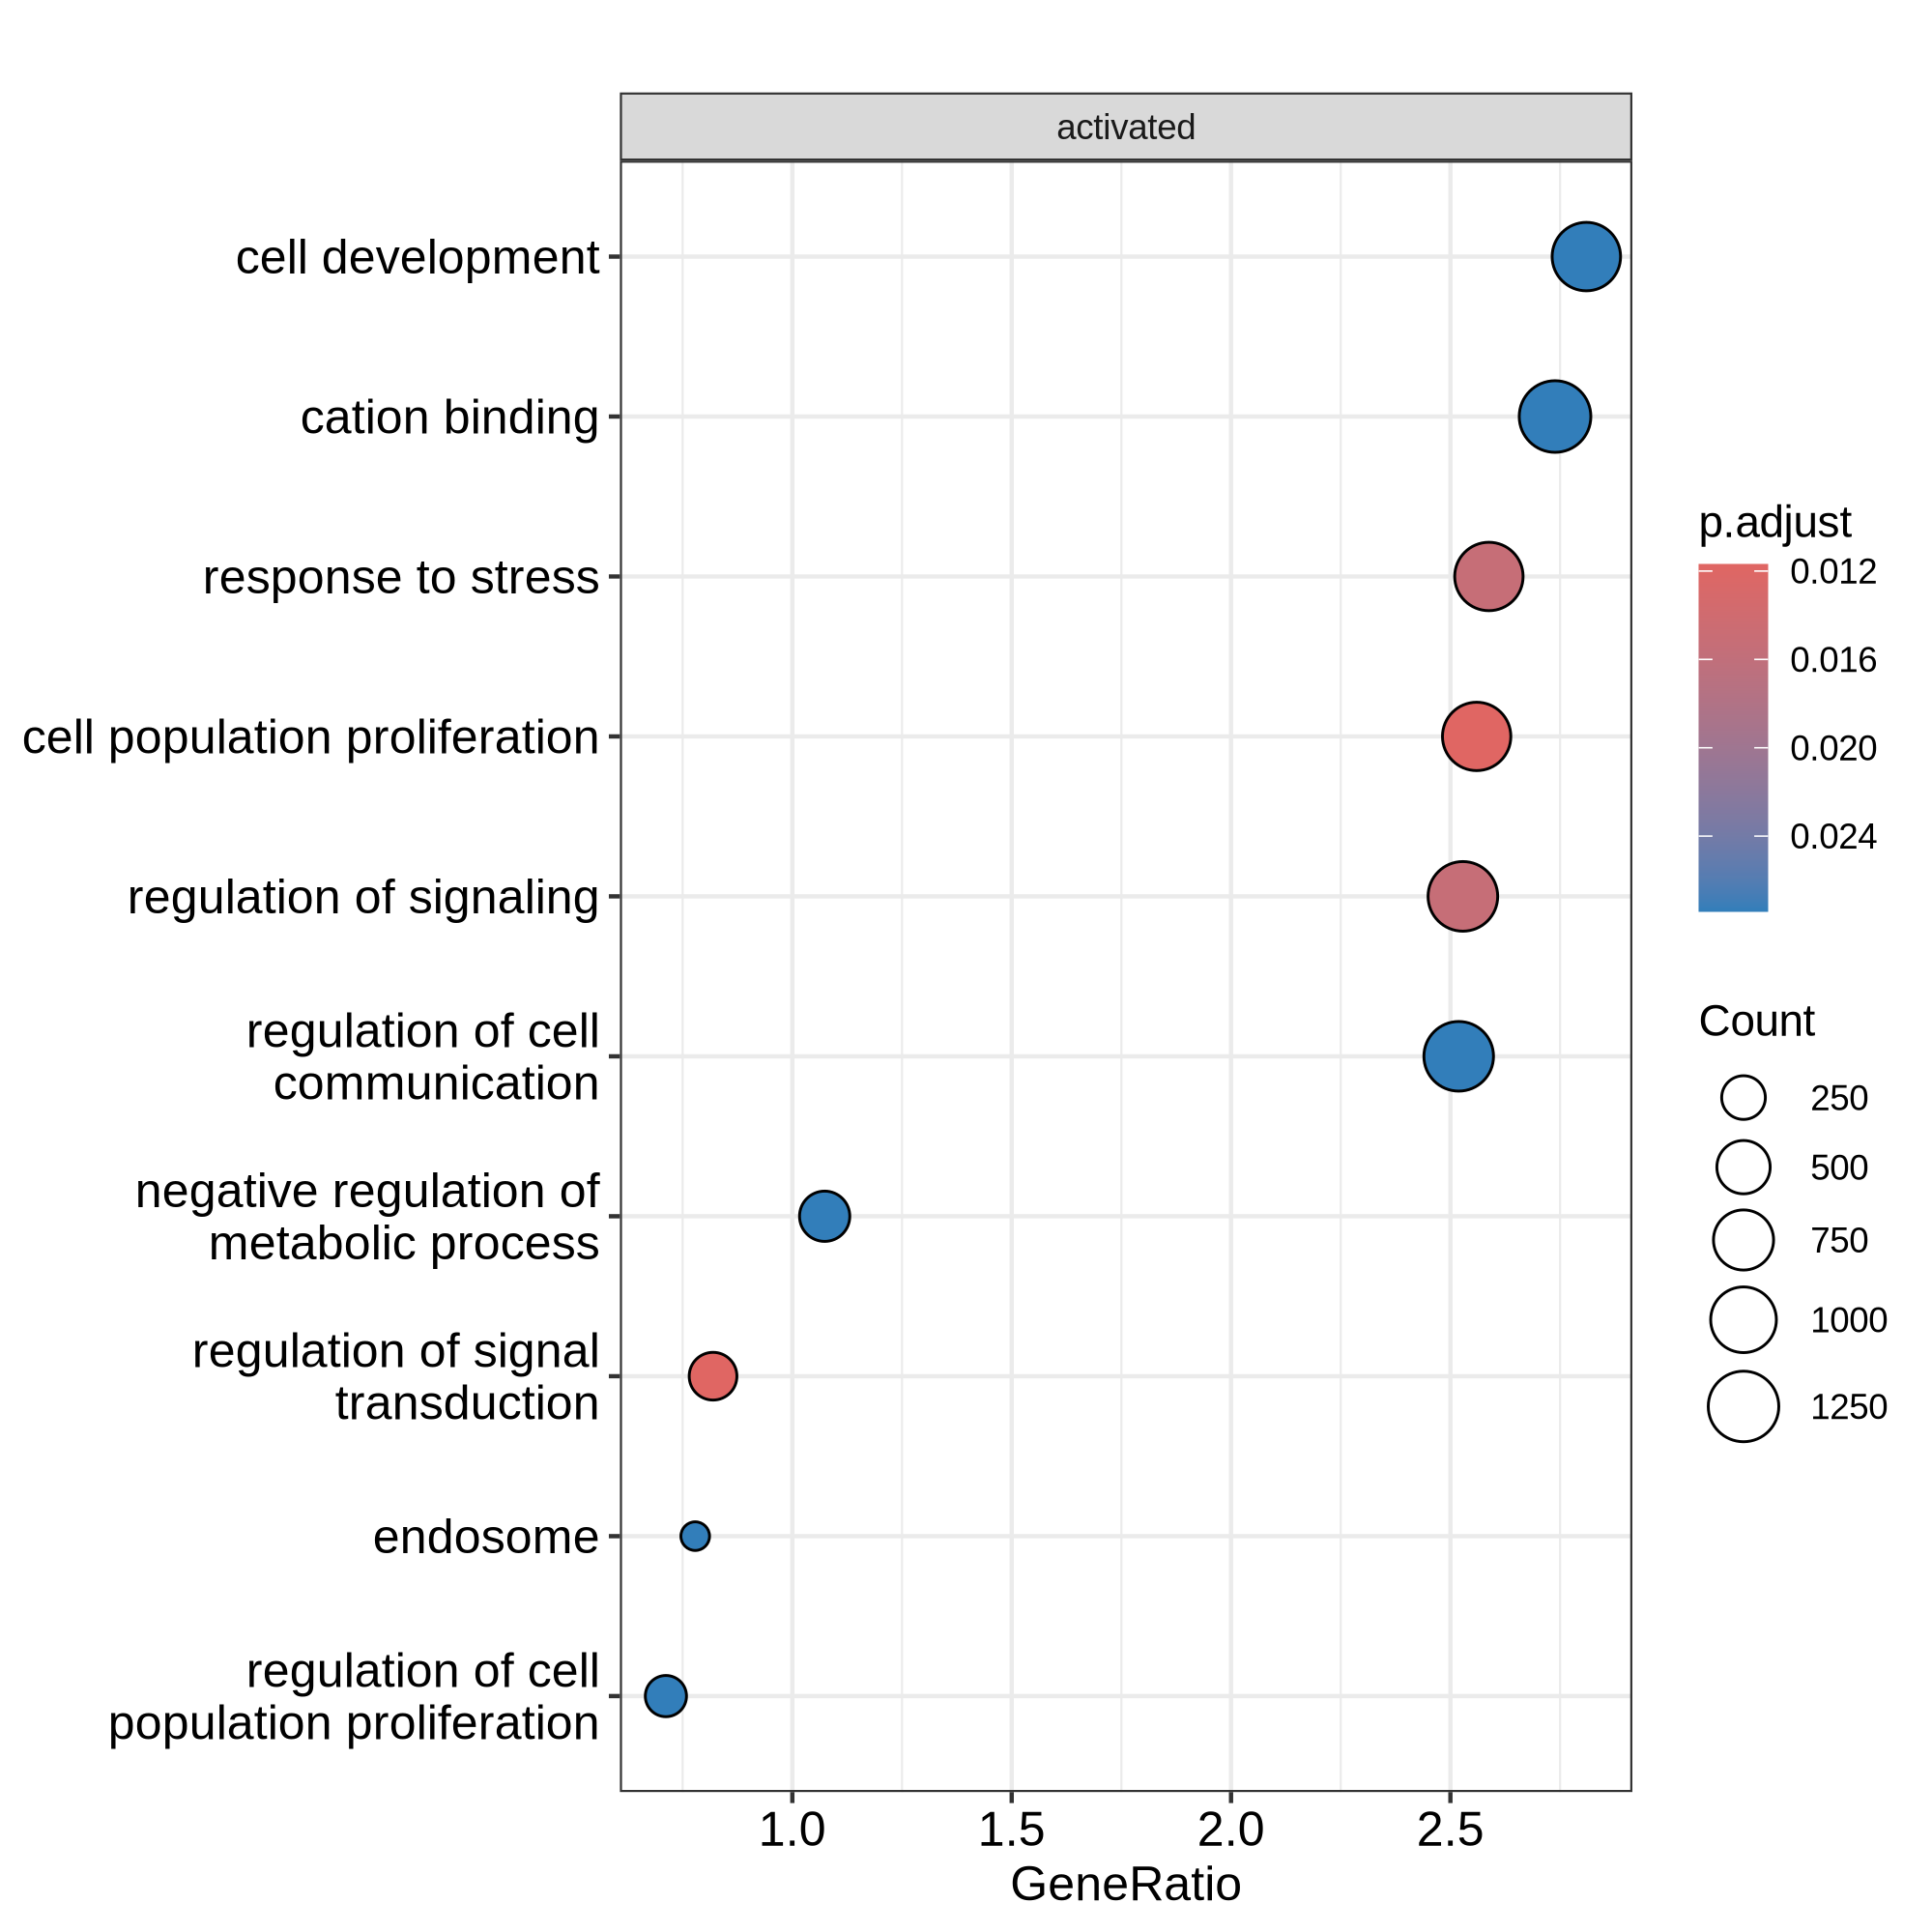
\includegraphics[width=\linewidth]{chapters/4_results_and_discussion/figures/dea/deseq2/esr1/dot.png}
            \caption{Functional enrichment of the host genes of the
                \glspl{crna} marked as significantly associated with \gls{esr1}
                expression.
                Only the ten highest-ranking terms are shown.
            }

            \label{fig:esr1_go_terms}
        \end{subfigure}
    \end{tabular}
    \caption{Results of differential expression analysis based on the
        association with \gls{esr1} expression (numeric contrast).
        Expression of the \gls{esr1} gene was determined using the nf-core/rnaseq
        pipeline\supercite{patel_nf-corernaseq_2024}.
        The following design formula was used: $\sim age + transgene + induction + drug
            + esr1$.
        The expression matrix containing all samples was tested for log2 fold changes
        with greater absolute values than 2.
        Benjamini-Hochberg correction\supercite{benjamini_controlling_1995} was used to
        adjust the $p$-values for multiple testing.
        \Glspl{crna} were considered significantly associated with \gls{esr1}
        expression if they had an adjusted $p$-value of less than 0.05.
    }
    \label{fig:dea_esr1}
\end{figure}

When looking at the result of the functional enrichment analysis, one has to
keep in mind that the expression of \glspl{crna} is not necessarily directly
linked to the expression of the host gene.
Furthermore \glspl{crna} might have a different function than their respective
host genes.

However, the results show that there are many \glspl{crna} that both originate
from host genes with a functional relation to estrogen and show a significant
association with the expression of \gls{esr1}.

In the following paragraphs I will discuss some of the most interesting
\gls{go} terms that were found in the functional enrichment analysis.

\paragraph{Developmental growth}
The \gls{go} term \textit{developmental growth} is associated with the growth
of a whole organism, a part of an organism, or a
cell\supercite{noauthor_quickgodevelopmental_nodate,binns_quickgo_2009}.
As discussed in \cref{sec:estrogen_signaling}, estrogen is known to promote
cell proliferation and differentiation in the breast tissue and other organs.
Thus, it is not surprising that the host genes of \glspl{crna} associated with
\gls{esr1} expression are enriched for this term.

\paragraph{Kinase binding}
Kinase binding is another area where estrogen receptors exert influence.
Estrogen receptors can interact with various kinases, which are essential for
signal transduction pathways that regulate cell proliferation and survival.
For instance, the activation of \gls{era} has been shown to involve the
phosphorylation of specific kinases, such as p38 MAPK, which is crucial for
mediating estrogen's effects on gene expression\supercite{lee_regulation_2002}.
This interaction between \glspl{er} and kinases underscores the importance of
kinase signaling in the regulation of estrogen-responsive genes, thereby
linking kinase binding to the broader context of estrogen receptor
signaling\supercite{campbell_phosphatidylinositol_2001}.
Moreover, the role of kinases in modulating \gls{er} activity highlights their
significance in the regulation of cell cycle processes and cellular
growth\supercite{lu_regulation_2003}.

\paragraph{Mitotic cell cycle and regulation of cell cycle process}
The mitotic cell cycle and its regulation are closely tied to estrogen receptor
signaling.
Estrogen has been shown to promote cell cycle progression, particularly in
hormone-responsive tissues.
The interaction of \glspl{er} with cell cycle regulators facilitates the
transition through various phases of the cell cycle, particularly in breast
cancer cells where \gls{era} is a key
player\supercite{drabovich_dynamics_2016}.
The regulation of genes involved in the cell cycle by estrogen underscores the
importance of \glspl{er} in maintaining proper cellular proliferation and
function\supercite{bjornstrom_mechanisms_2005}.
Additionally, studies have demonstrated that estrogen can induce the expression
of cyclins and cyclin-dependent kinases, which are critical for cell cycle
progression, further linking \gls{er} expression to the regulation of the cell
cycle\supercite{g_widespread_2009}.

\subsection{\Glsfmtshortpl{crna} associated with \glsfmtlong{tam} treatment}

Next, the differential expression analysis was performed to identify
\glspl{crna} associated with \gls{tam} treatment.
For this purpose, all untreated samples were used as the control group, and all
samples treated with \gls{tam} were used as the treatment group.
The results of the differential expression analysis using DESeq2 and
\gls{ciriquant} are shown in \cref{fig:tamoxifen_volcano}.

\begin{figure}[H] \begin{tabular}{cc} \begin{subfigure}{0.5\textwidth}
                 \centering

                 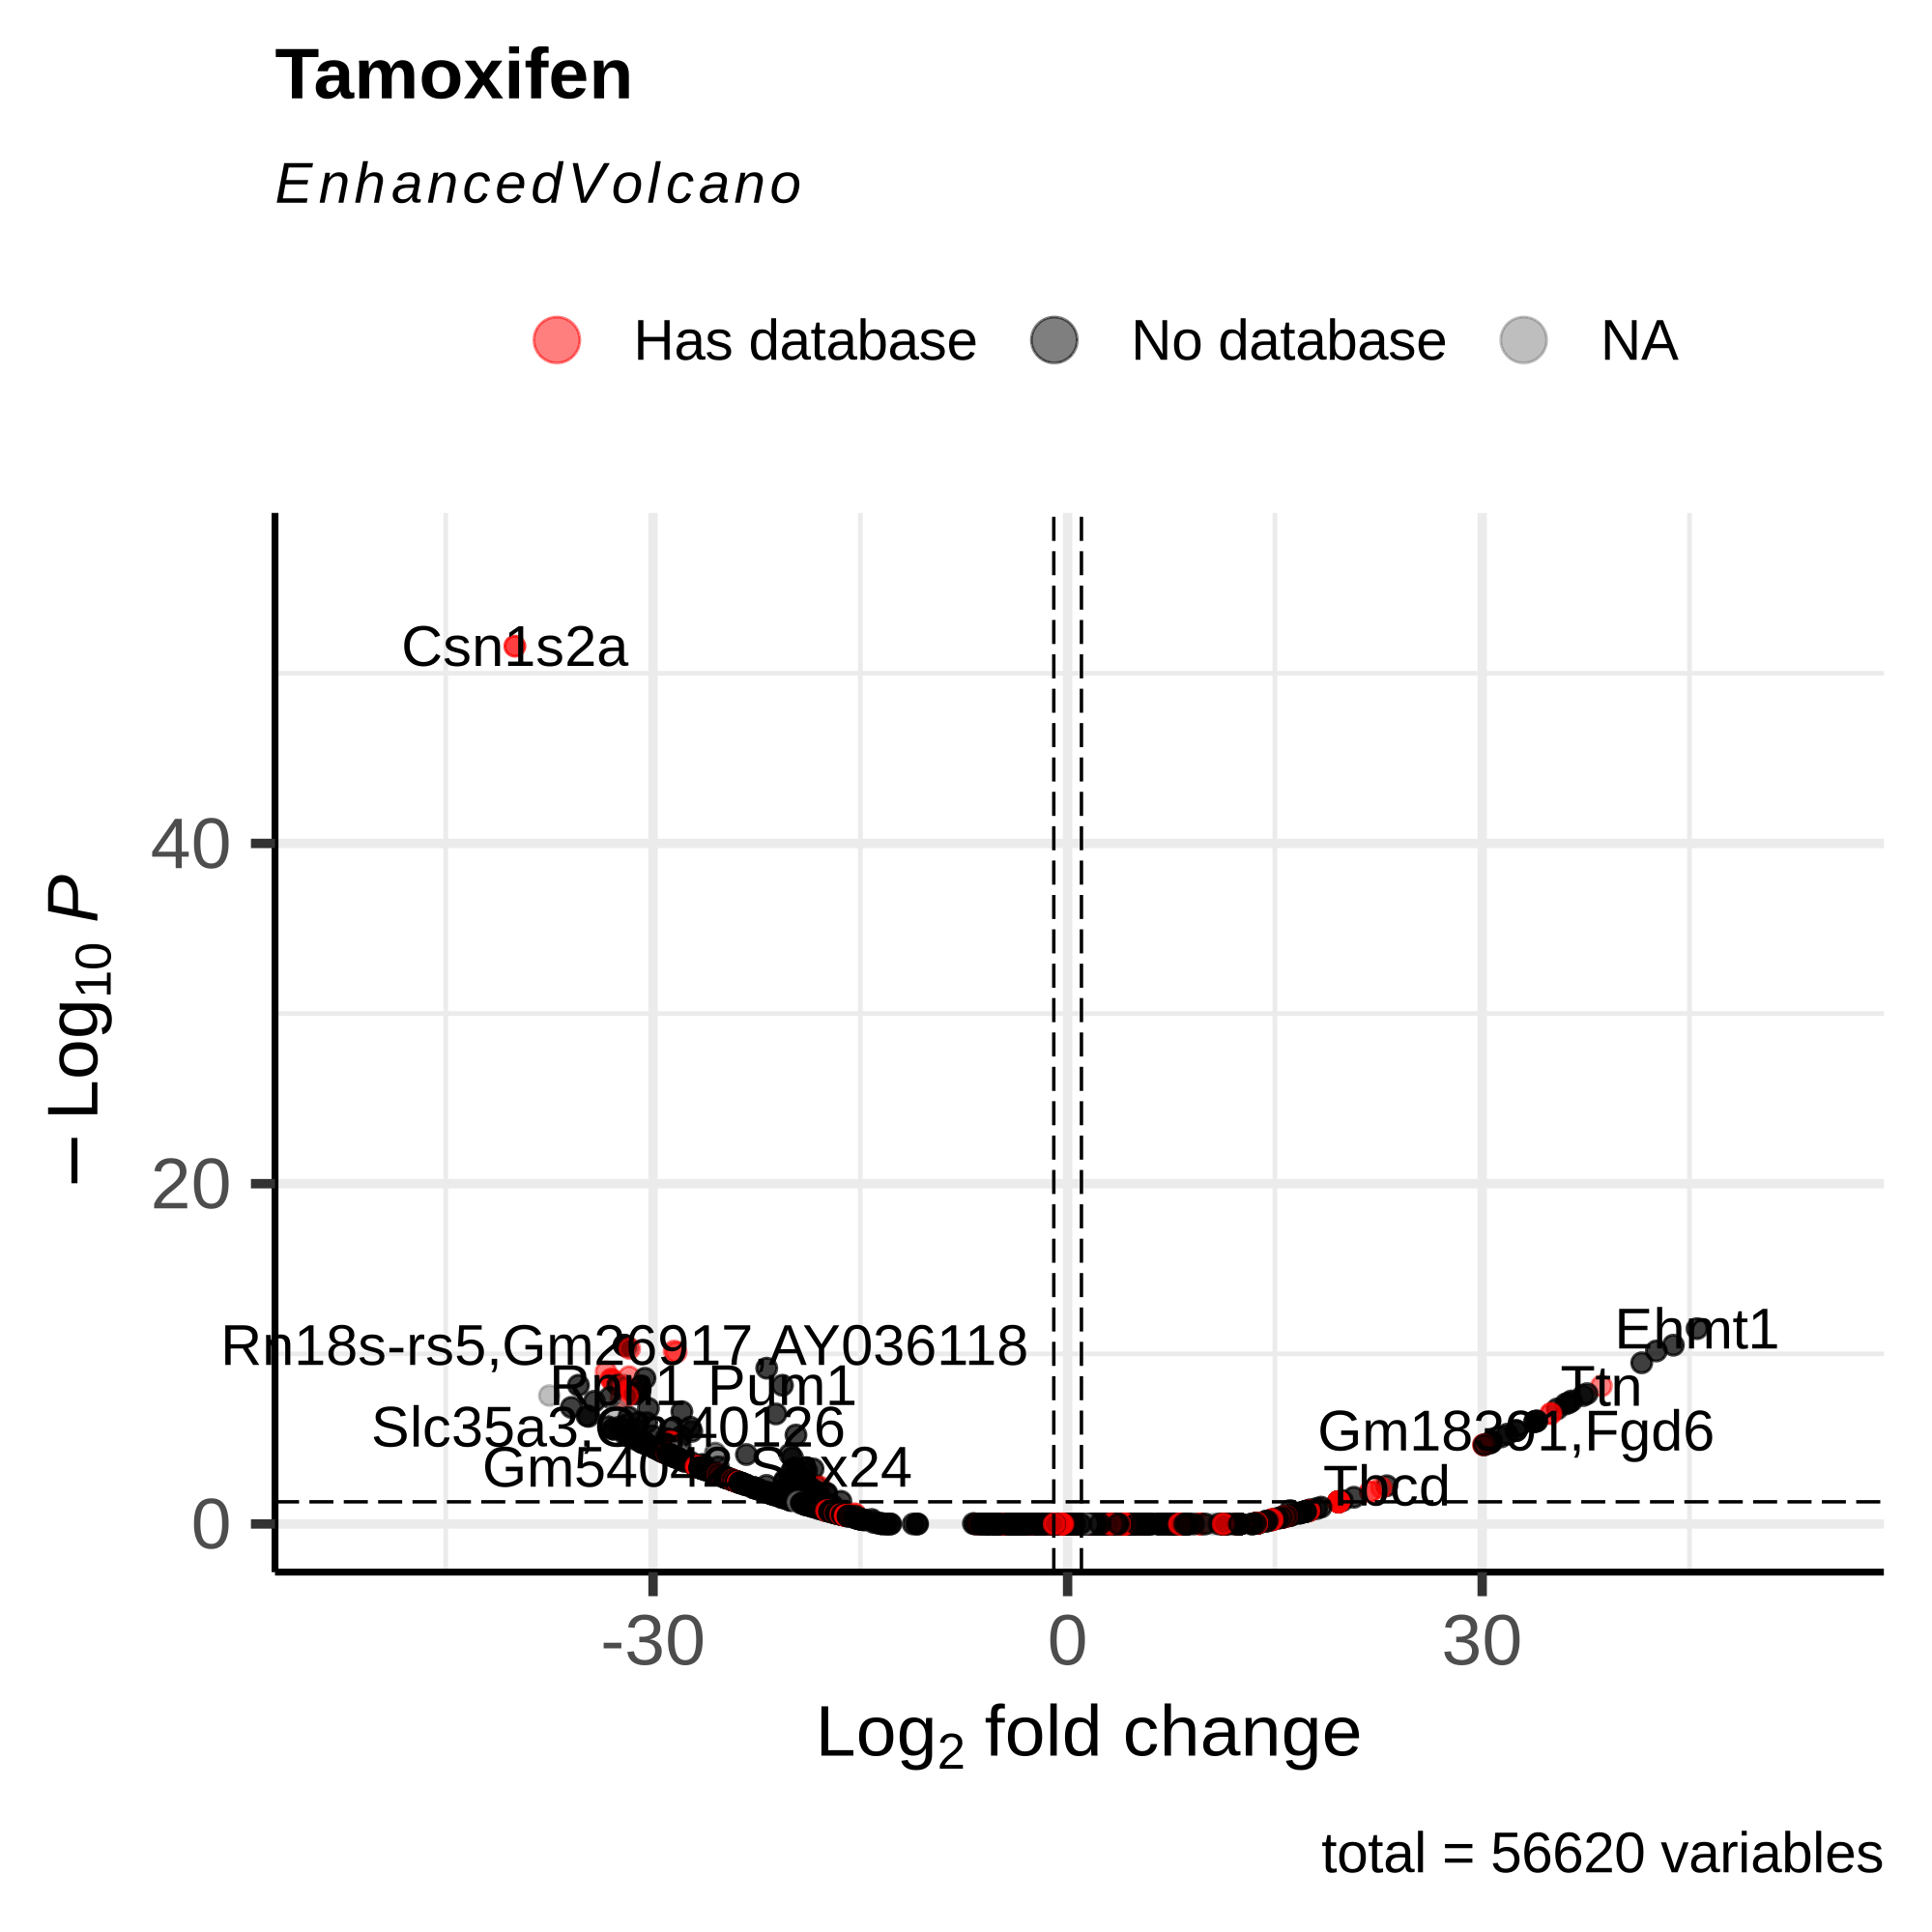
\includegraphics[width=\linewidth]{chapters/4_results_and_discussion/figures/dea/deseq2/tamoxifen/volcano.png}
                 \caption{Volcano plot illustrating the differential expression
                     results obtained
                     using DESeq2.
                     The following design formula was used: $\sim age + transgene + induction +
                         drug$.
                     The expression matrix was tested for log2 fold changes with greater absolute
                     values than 2.
                 }
                 \label{fig:tamoxifen_volcano_deseq2}
             \end{subfigure}
        \begin{subfigure}{0.5\textwidth}
            \centering

            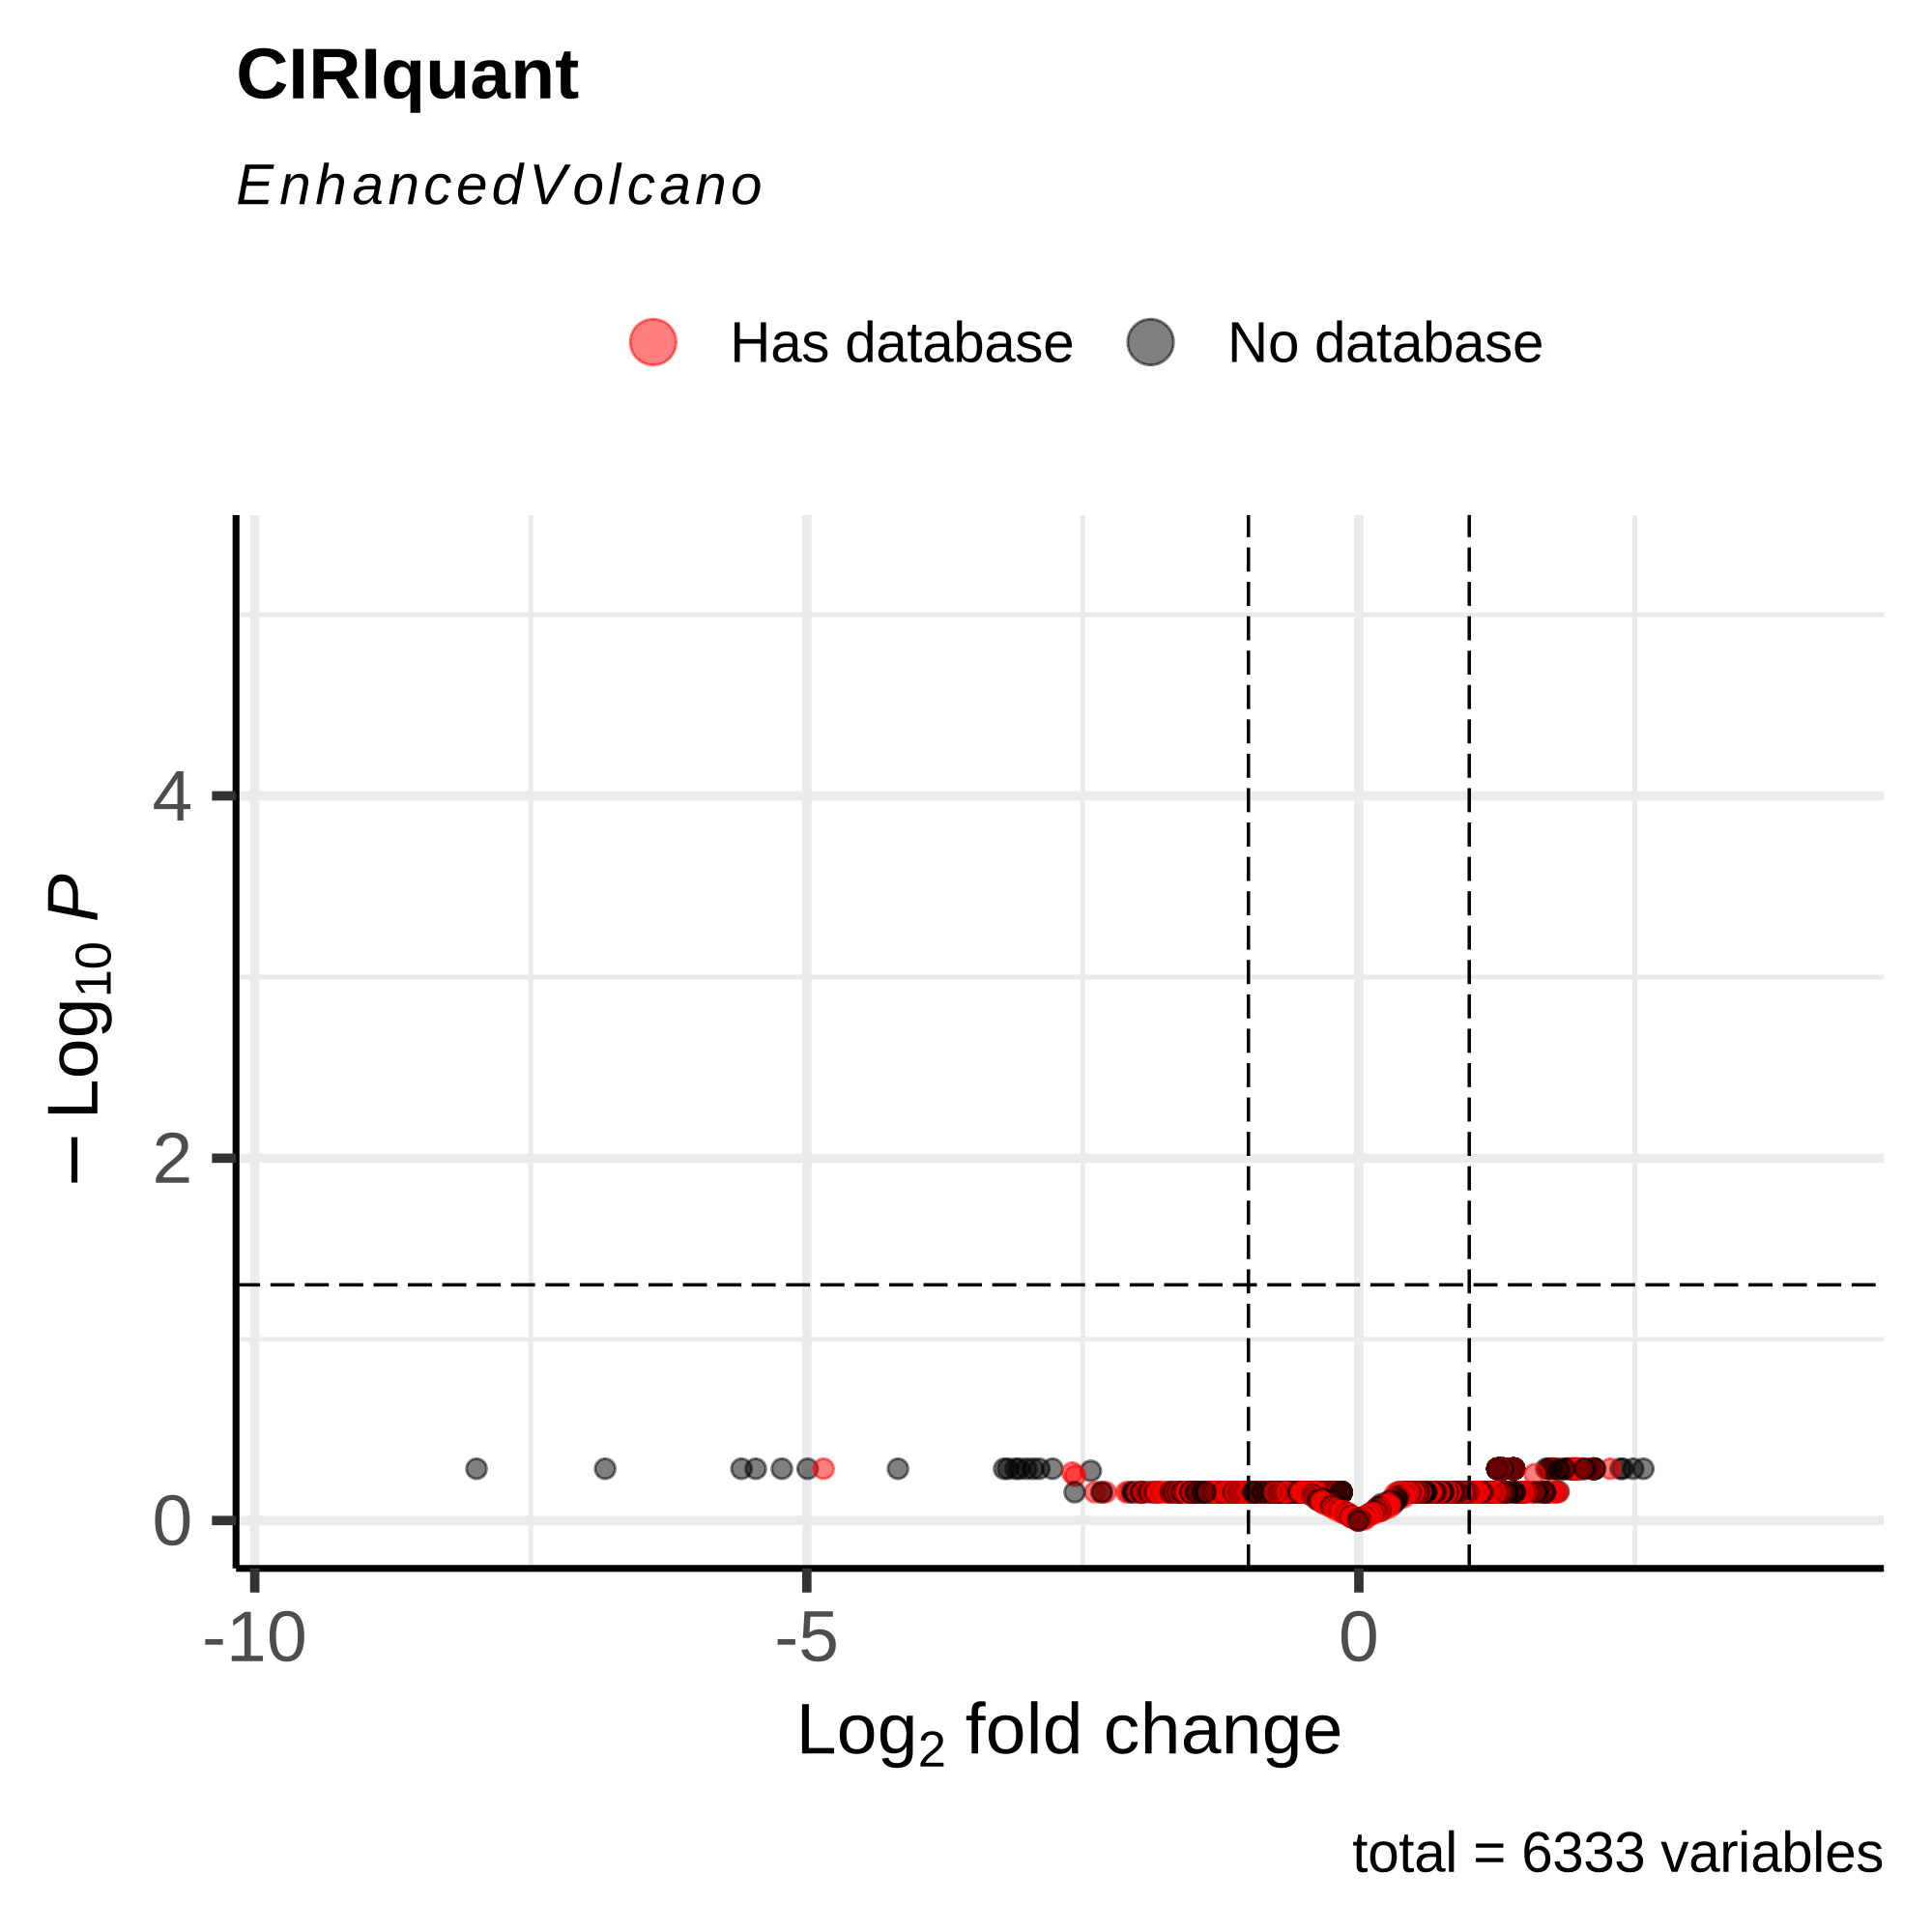
\includegraphics[width=\linewidth]{chapters/4_results_and_discussion/figures/dea/ciriquant/tamoxifen/volcano.png}
            \caption{Volcano plot illustrating the differential expression
                results obtained using \gls{ciriquant}.
                Samples without treatment were used as the control group, and samples treated
                with \gls{tam} were used as the treatment group.
            }
            \label{fig:tamoxifen_volcano_ciriquant}
        \end{subfigure}

    \end{tabular}
    \caption{Results of differential expression analysis comparing untreated
        samples with samples treated using \gls{tam} (binary contrast).
        Benjamini-Hochberg correction\supercite{benjamini_controlling_1995} was used to
        adjust the $p$-values for multiple testing.
        \Glspl{crna} were considered significantly associated with \gls{tam}
        treatment if they had an adjusted $p$-value of less than 0.05.
    } \label{fig:tamoxifen_volcano} \end{figure}

While DESeq2 identified a total of x significantly differentially expressed
\glspl{crna} (\cref{fig:tamoxifen_volcano_deseq2}), \gls{ciriquant} did not
find any \glspl{crna} to be significantly associated with \gls{tam} treatment
(\cref{fig:tamoxifen_volcano_ciriquant}).
This indicates that \gls{ciriquant} might be more conservative in its approach
to differential expression analysis compared to DESeq2.

When looking closer at the results obtained using DESeq2, it is evident that
the majority of the significantly differentially expressed \glspl{crna} have a
negative log $p$-value of less than 15 However, there is one outlier with a
negative log $p$-value of approximately 50.
This \gls{crna} might be of particular interest for further investigation.
Its \gls{bsj} is located on chromosome 5 and reaches from position 87925915 to
87926842.
The host gene of this \gls{crna} is \textit{Csn1s2a}.

\subsection{\Glsfmtshortpl{crna} associated with \gls{let} treatment}

The differential expression analysis was also performed to identify
\glspl{crna} associated with \gls{let} treatment.
The same setup as in the analysis of \gls{tam} treatment was used.

\begin{figure}[H] \begin{tabular}{cc} \begin{subfigure}{0.5\textwidth}
                 \centering

                 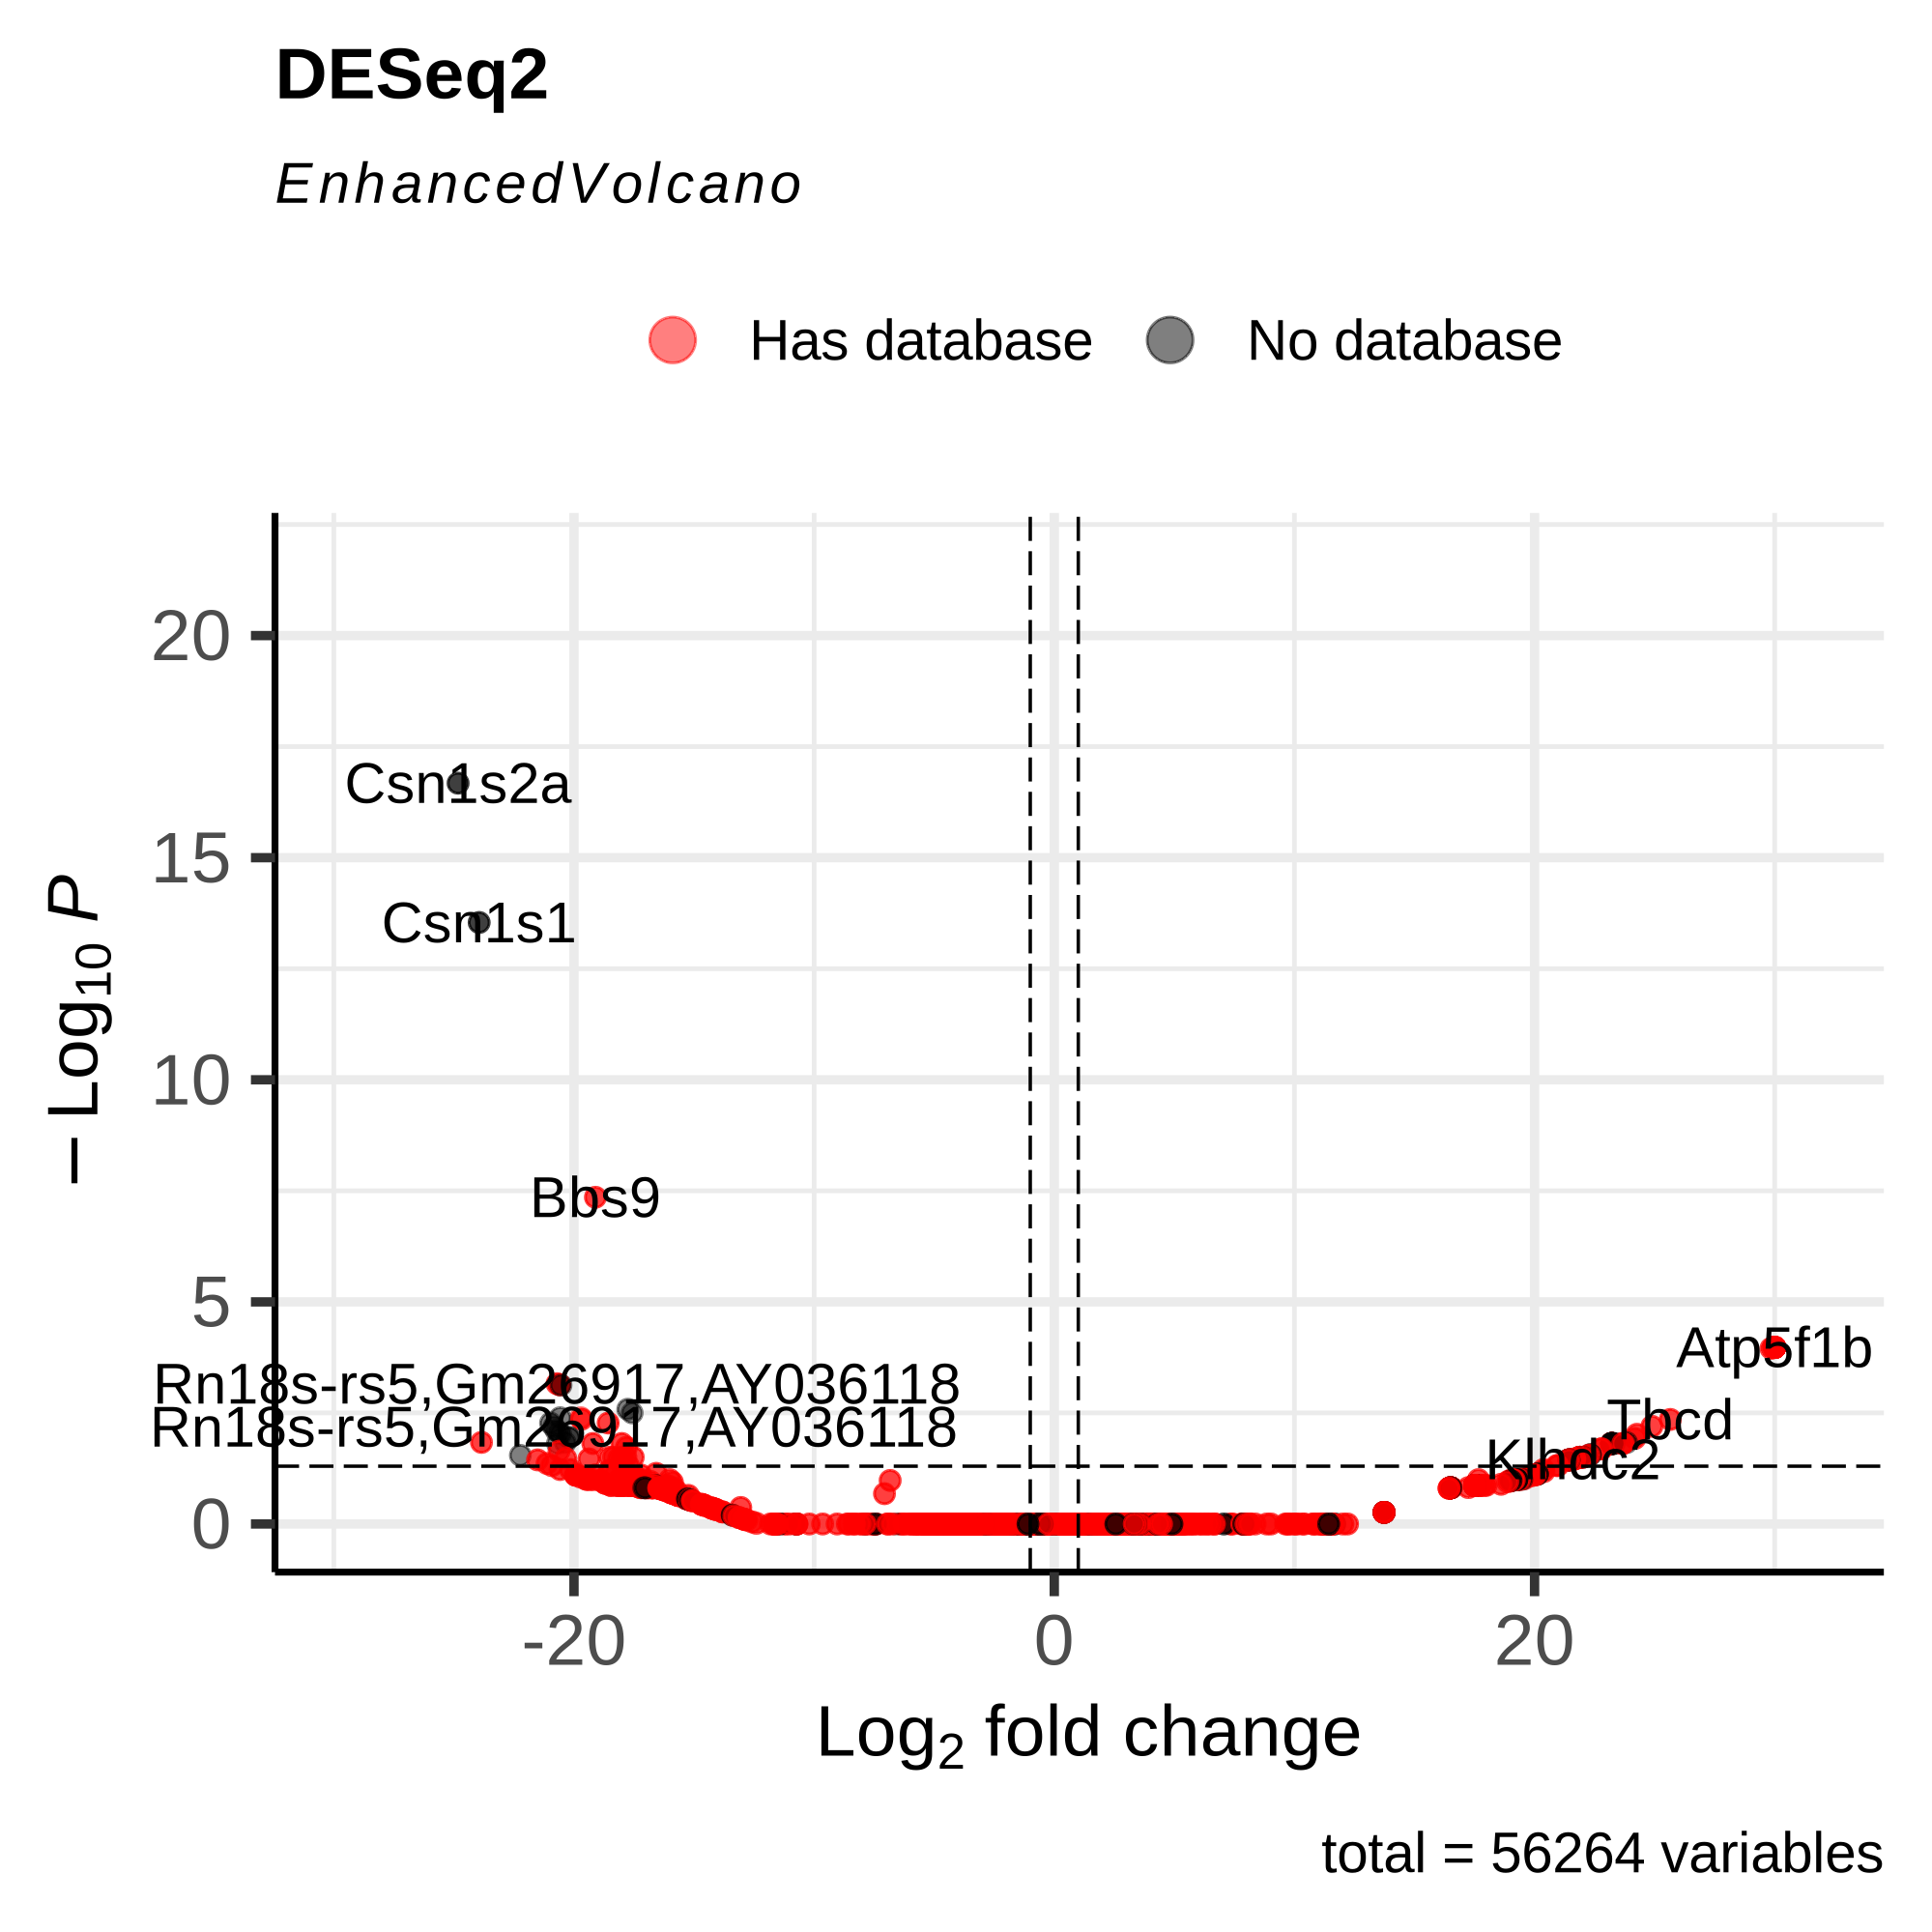
\includegraphics[width=\linewidth]{chapters/4_results_and_discussion/figures/dea/deseq2/letrozole/volcano.png}
                 \caption{Volcano plot illustrating the differential expression
                     results obtained
                     using DESeq2.
                     The same setup as in \cref{fig:tamoxifen_volcano_deseq2} was used.
                 }
                 \label{fig:letrozole_volcano_deseq2}
             \end{subfigure}
        \begin{subfigure}{0.5\textwidth}
            \centering

            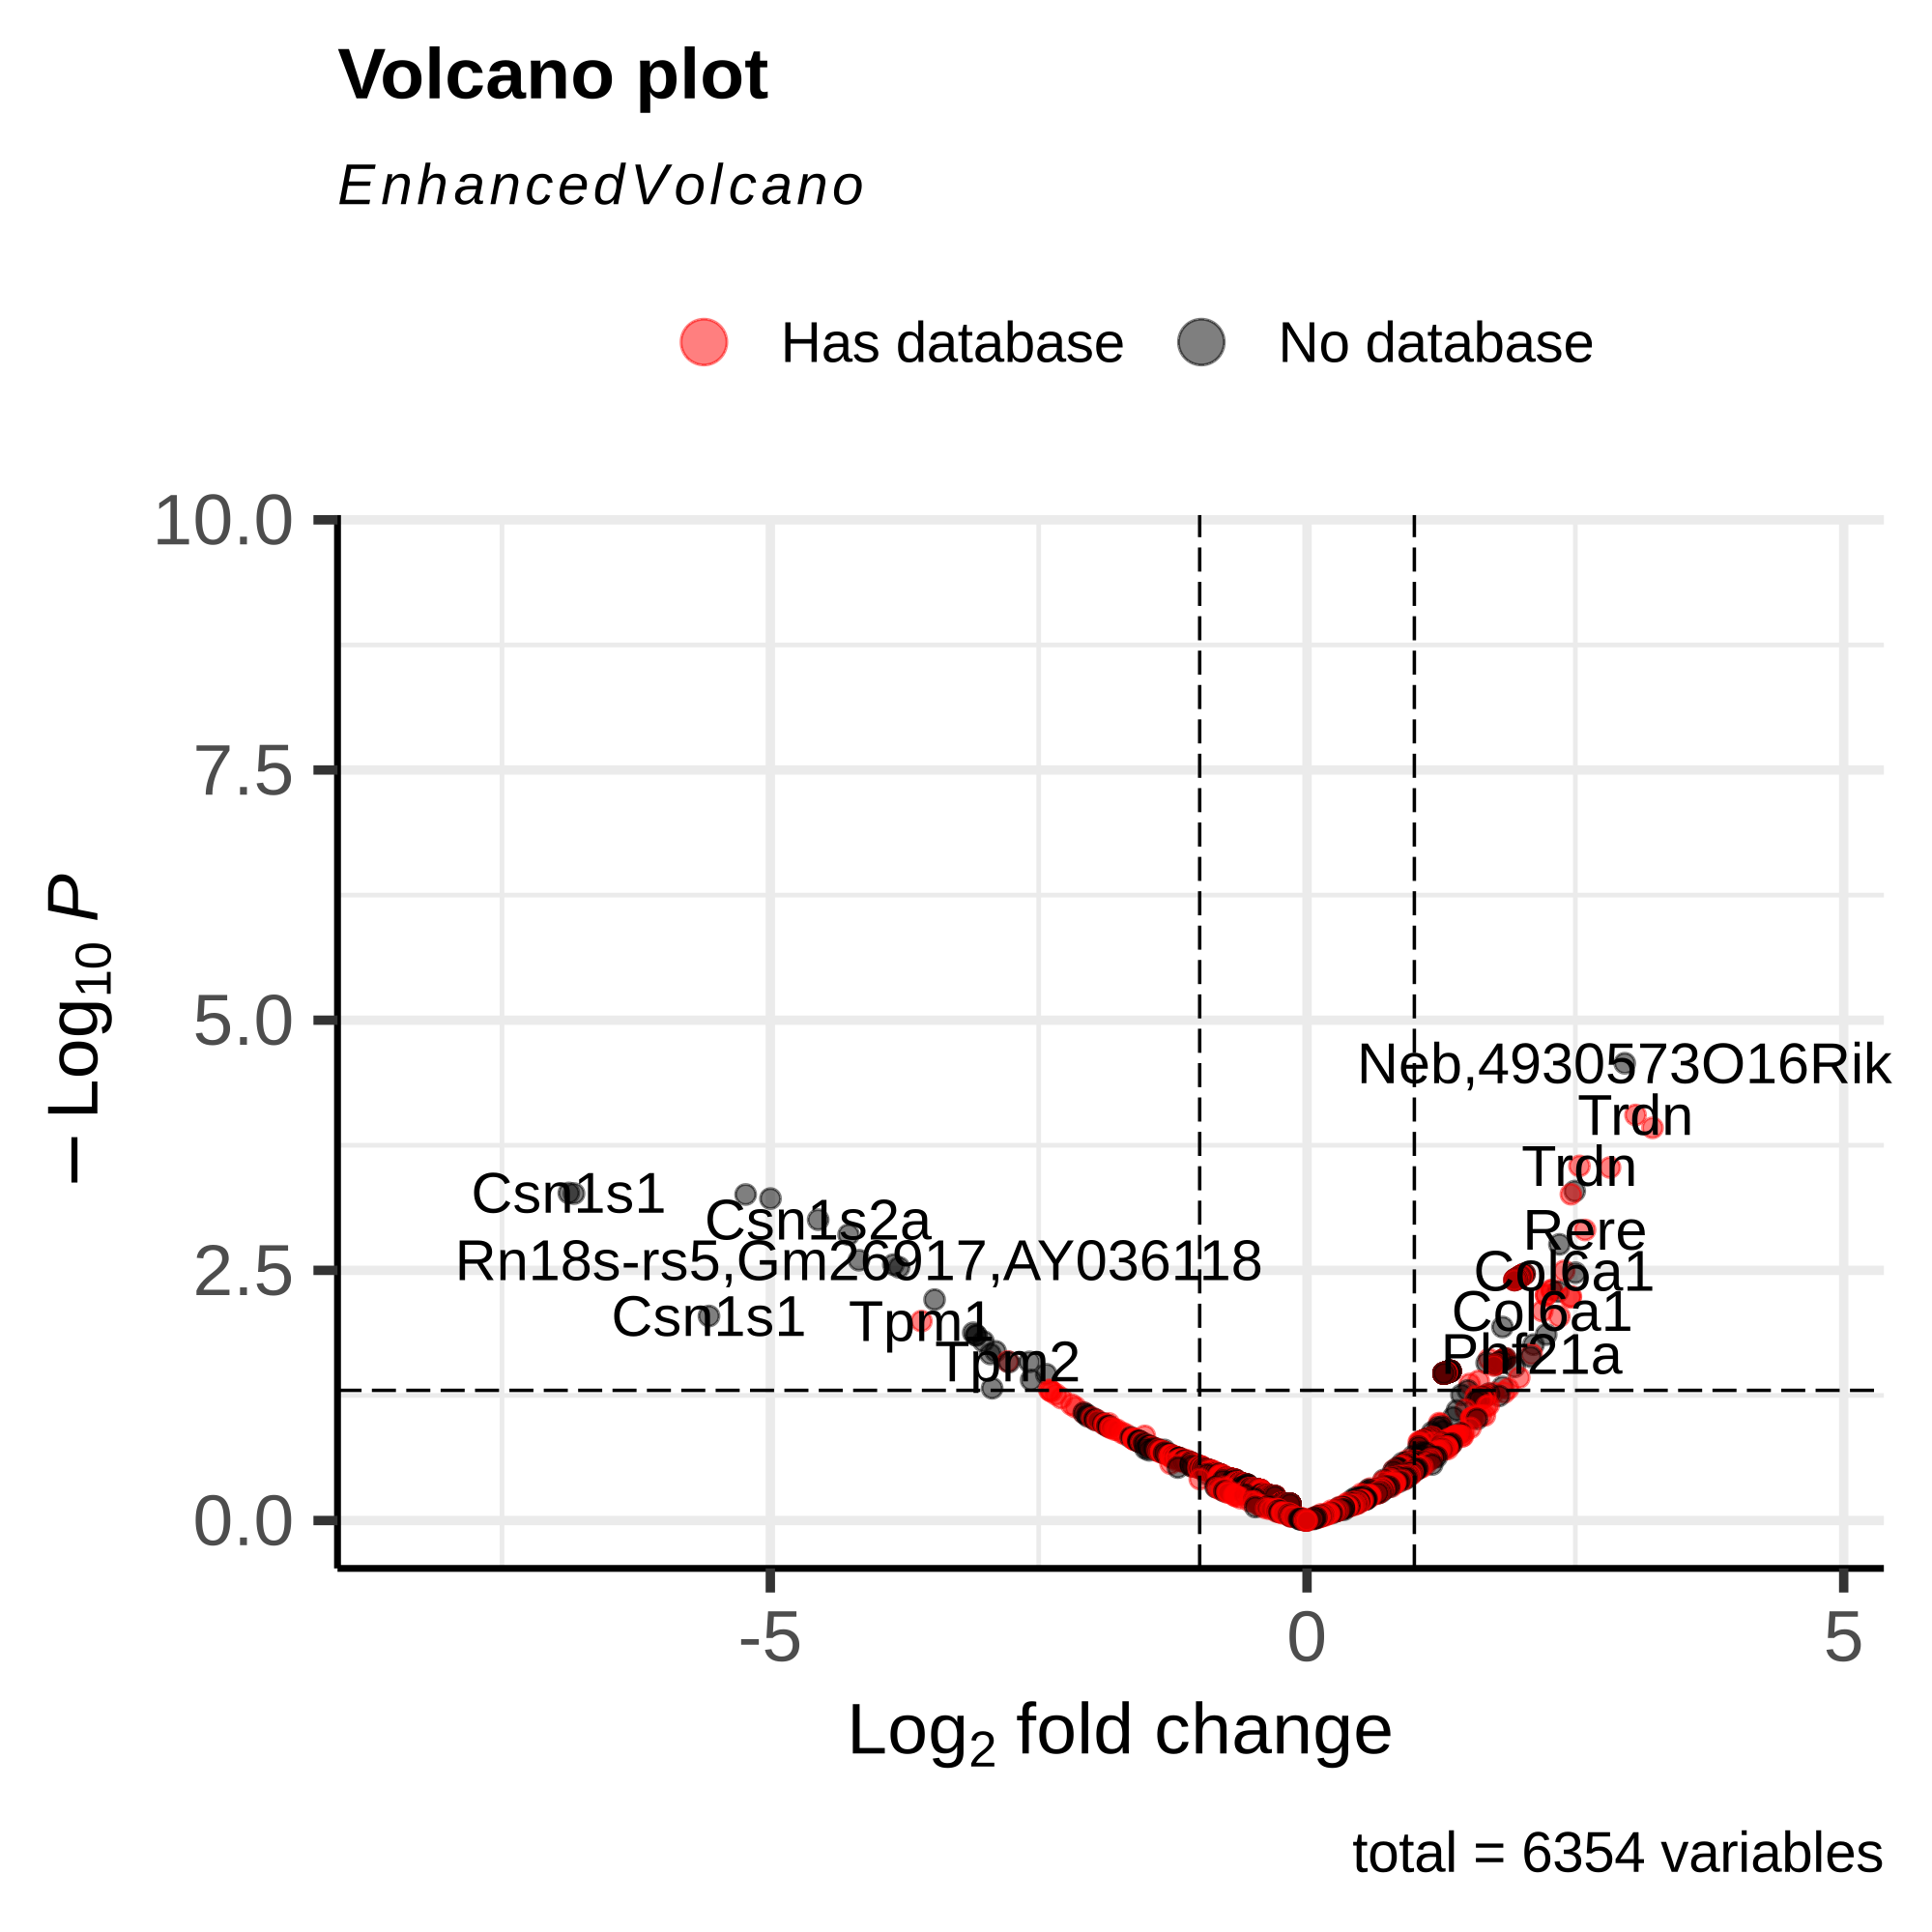
\includegraphics[width=\linewidth]{chapters/4_results_and_discussion/figures/dea/ciriquant/letrozole/volcano.png}
            \caption{Volcano plot illustrating the differential expression
                results obtained using \gls{ciriquant}.
            }
            \label{fig:letrozole_volcano_ciriquant}
        \end{subfigure} &

    \end{tabular}
    \caption{Results of differential expression analysis using the same
        approach as in
        \cref{fig:tamoxifen_volcano}, but comparing samples treated with
        \gls{let}
        to untreated samples.
    }
    \label{fig:letrozole_volcano}
\end{figure}

Similar to the results obtained for \gls{tam} treatment, DESeq2 identified a
large number of significantly differentially expressed \glspl{crna} in the
analysis of \gls{let} treatment, while \gls{ciriquant} did not find any.

When looking at the distribution of the significant \glspl{crna} in the volcano
plot obtained using DESeq2 (\cref{fig:letrozole_volcano_deseq2}), again most of
the \glspl{crna} have negative log $p$-values below a certain threshold.
This time, there are three outliers.
Most interestingly, the most significant \gls{crna} is the exact same as the
one found in the analysis of \gls{tam} treatment.
An overview of the outliers from both analyses is shown in \cref{tab:outliers}.

\begin{table}[H] \centering \begin{tabular}{ccccc} \hline Location   &
               Host gene
                                         & Adj. $p$-val. (\gls{tam})
                                         &
               Adj. $p$-val. (\gls{let}) & Has DB entry
               \\ \hline
               chr5:87925915-87926842    & \textit{Csn1s2a}
                                         &
               2.554e-52
                                         & 2.105e-17
                                         & No
               \\
               chr5:87817372-87821140    & \textit{Csn1s1}
                                         & not
               significant               & 2.876e-14
                                         & No
               \\
               chr9:22555041-22570441    & \textit{Bbs9}
                                         & not
               significant               & 4.415e-08
                                         & Yes
               \\
               \hline
    \end{tabular} \caption{Overview of the outliers found in the differential
        expression analysis of \gls{tam} and \gls{let} treatment.
        The \gls{bsj} location, host gene, and adjusted $p$-values are shown.
    }
    \label{tab:outliers}
\end{table}

The fact that the same \gls{crna} was found to be significantly associated with
both \gls{tam} and \gls{let} treatment is intriguing.
Furthermore,there are two other \glspl{crna} that are significantly associated
with \gls{let} treatment, but not with \gls{tam} treatment.
From now on, I will refer to these three \glspl{crna} using their host gene
names: \textit{circ-Csn1s2a}, \textit{circ-Csn1s1}, and \textit{circ-Bbs9}.

\subsection{Investigating the expression patterns of the candidate
    \glsfmtshortpl{crna}}

In order to get a better understanding of the expression patterns that led to
the identification of the three candidate \glspl{crna}, the expression levels
of these \glspl{crna} were visualized across all samples.

\begin{figure}[H] \centering

    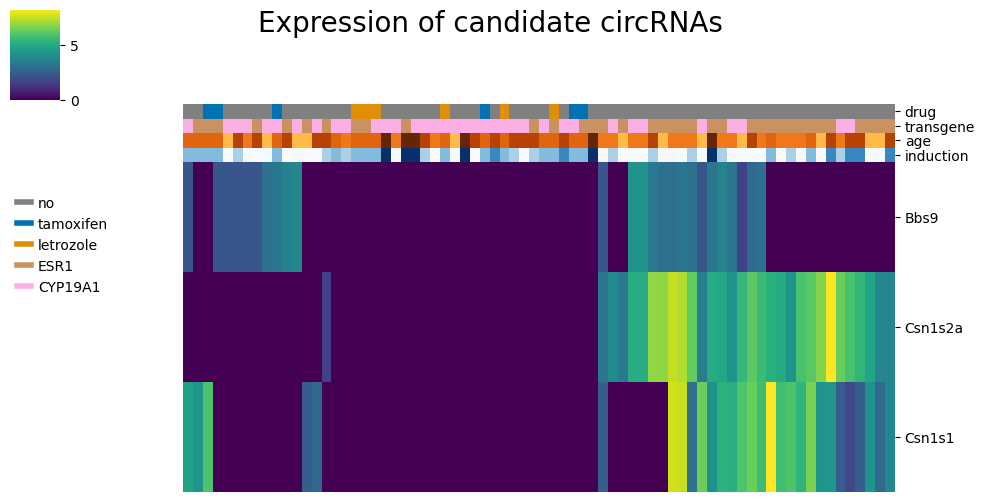
\includegraphics[width=\textwidth]{chapters/4_results_and_discussion/figures/heatmap.png}
    \caption{Clustermap showing the expression levels of the candidate
        \glspl{crna} \textit{circ-Csn1s2a}, \textit{circ-Csn1s1}, and
        \textit{circ-Bbs9} across all samples.
        The expression values were log-normalized with a pseudo count of 1.
        Covariates are shown on the top of the plot.
        For numerical covariates, darker colors indicate higher values.
    }
    \label{fig:candidate_heatmap}
\end{figure}

The clustermap in \cref{fig:candidate_heatmap} shows the expression levels of
the three candidate \glspl{crna} across all samples.
While the expression all three \glspl{crna} have portions of samples with high
expression, all of them are lowly expressed in almost all treated samples.
However, there are also many untreated samples with low expression levels.
Interestingly, these samples are mostly from cohorts with the \gls{cyp19}
transgene.

In summary, it looks like untreated samples with the \gls{esr1} transgene have
higher expression levels of the candidate \glspl{crna} compared to samples that
have the \gls{cyp19} transgene or have been treated with \gls{tam} or
\gls{let}.
